\documentclass{article}
\usepackage{amsmath, amssymb, amsthm, graphicx}

% Define custom theorem styles
\newtheoremstyle{remarkstyle} % name
  {\topsep}   % Space above
  {\topsep}   % Space below
  {}          % Body font
  {}          % Indent amount
  {\bfseries} % Theorem head font
  {.}         % Punctuation after theorem head
  {.5em}      % Space after theorem head
  {\thmname{#1}\thmnumber{ #2}\thmnote{ (#3)}} % Theorem head spec (empty for remark)
\theoremstyle{remarkstyle}
\newtheorem*{remark}{Remark}

\newtheoremstyle{examplestyle} % name
  {\topsep}   % Space above
  {\topsep}   % Space below
  {}          % Body font
  {}          % Indent amount
  {\bfseries} % Theorem head font
  {.}         % Punctuation after theorem head
  {.5em}      % Space after theorem head
  {\thmname{#1}\thmnumber{ #2}\thmnote{ (#3)}} % Theorem head spec (empty for example)
\theoremstyle{examplestyle}
\newtheorem*{example}{Example}

\newtheoremstyle{definitionstyle} % name
  {\topsep}   % Space above
  {\topsep}   % Space below
  {}          % Body font
  {}          % Indent amount
  {\bfseries} % Theorem head font
  {.}         % Punctuation after theorem head
  {.5em}      % Space after theorem head
  {\thmname{#1}\thmnumber{ #2}\thmnote{ (#3)}} % Theorem head spec (empty for definition)
\theoremstyle{definitionstyle}
\newtheorem*{definition}{Definition}

\newtheoremstyle{lemmastyle} % name
  {\topsep}   % Space above
  {\topsep}   % Space below
  {}          % Body font
  {}          % Indent amount
  {\bfseries} % Theorem head font
  {.}         % Punctuation after theorem head
  {.5em}      % Space after theorem head
  {\thmname{#1}\thmnumber{ #2}\thmnote{ (#3)}} % Theorem head spec (empty for lemma)
\theoremstyle{lemmastyle}
\newtheorem*{lemma}{Lemma}

\newtheoremstyle{theoremstyle} % name
  {\topsep}   % Space above
  {\topsep}   % Space below
  {\itshape}  % Body font
  {}          % Indent amount
  {\bfseries} % Theorem head font
  {.}         % Punctuation after theorem head
  {.5em}      % Space after theorem head
  {\thmname{#1}\thmnumber{ #2}\thmnote{ (#3)}} % Theorem head spec
\theoremstyle{theoremstyle}
\newtheorem*{theorem}{Theorem}

\begin{document}

% Content from IE - Teorico 25bis.md converted to LaTeX

\begin{remark}
Entonces la convención es mantener el ET I bajo control, por lo tanto como se eligen las hip. nula y alternativa en el problema particular que estemos analizando. Es una decisión en términos de lo que se considere el interés en el fenómeno bajo estudio. Veamos el siguiente ejemplo.
\end{remark}

\begin{example}
Supongamos que estudiamos una nueva droga que deseamos saber si aumenta la tasa de recuperación resp. de tratamientos anteriores. Supongamos que de la experiencia con las drogas anteriores, la tasa de recuperación es $\theta_0 = 0.3$.
El científico que descubre la nueva droga quiere minimizar el error de decir que la nueva droga es mejor cuando eso no ocurre (1) .
Hay dos posibles errores que uno puede cometer:
\begin{itemize}
    \item "Decir que la nueva droga es mejor que la anterior cuando esto no ocurre"
    \item "Decir que la nueva droga es igual que las anteriores cuando esto no ocurre"
\end{itemize}

Equivalentemente:
\begin{itemize}
    \item Decir que $\theta > 0.3$ cuando $\theta = 0.3$ (2)
    \item Decir que $\theta = 0.3$ cuando $\theta > 0.3$
\end{itemize}

En términos del interés del científico (1) , entonces lo que planteamos como problema de hipótesis es:
\[H_0: \theta=0.3 \text{ vs } H_1: \theta>0.3\]
que es equivalente a rechazar $H_0$ (decir que $\theta > 0.3$) siendo $H_0$ verdadera (2) (o sea cdo la nueva droga no es más eficiente).

Se realiza entonces una experiencia donde se toma una muestra aleatoria de la población enferma, donde se administra la nueva droga. Se obtiene una muestra $X=(X_1, \dots, X_n)^t$ donde $X_i \sim \text{Bi}(1, \theta)$, $i=1, \dots, n$ independientes. Sea $S = \sum_{i=1}^n X_i$ el número de pacientes recuperados con la nueva droga, $S \sim \text{Bi}(n, \theta)$. 
Para plantear una región de rechazo para construir el test, observamos que la f.d.a de $S$, $P_\theta(S \le k) = F_\theta(k)$ es decreciente en $\theta \in (0,1)$ para cada $k$ fijado. (es un resultado que se puede probar).
Luego, $S$ tiende a producir valores más grandes a medida que $\theta$ crece, con lo cual podríamos decir: Rechazar $H_0$ si $S$ es más "grande" de lo que hubieramos esperado por azar si $H_0: \theta=0.3$ es verdadera. Entonces la región de rechazo resultaría: $C = \{x\in \Omega_{X}: S(x) > k\}$, con $k$ a determinar, y el test resultaría:
\[ \phi(x) = I_{\{k, k+1, \dots, n\}}(S)= \begin{cases} 1 & \text{si } x \in C \\ 0 & \text{si } x \notin C \end{cases} \]
$k$ se determina usando la condición de nivel $\alpha$:
\[ \beta_\phi(\theta_0) =\sup_{P\in \mathcal{P}_{0}}E_{P}(\phi(x))= E_{\theta_0}[\phi] = P_{\theta_0}(S > k) \le \alpha \]
(supremo se simplifica por que hay un solo elemento en el conjunto $\mathcal{P}_{0}$) 
La idea es determinar "$k$" de forma que $P_{\theta_0}(S > k)$ sea "chico" (porque entonces es "chico" el ETI que queremos controlar).

Para fijar ideas, supongamos en nuestro caso que $n=10$ y $\theta_0=0.3$
Al buscar en tablas o con un paquete estadístico vemos por ejemplo que
Tomando $k=5$ resulta que
\[ P_{0.3}(S > 5) = 0.0473 \]
En este caso, como $\mathcal{P}_0 = \{P_{0.3}\}$, el supremo se alcanza en el único elemento del conjunto:
\[ \sup_{P \in \mathcal{P}_0} E_P[\phi(\underline{X})] = E_{0.3}[\phi(\underline{X})] = P_{0.3}(S > 5) \]
"$k$" recibe el nombre de \textbf{valor crítico}. Luego, el test es definido por
\[ \phi(X_1, \dots, X_n) = \begin{cases} 1 & \text{si } S > 5 \\ 0 & \text{si } S \le 5 \end{cases} \]
y $\{S > 5\}$ es la \textbf{región crítica}, produce un test de tamaño $0.0473$.

Ademas Notar
% 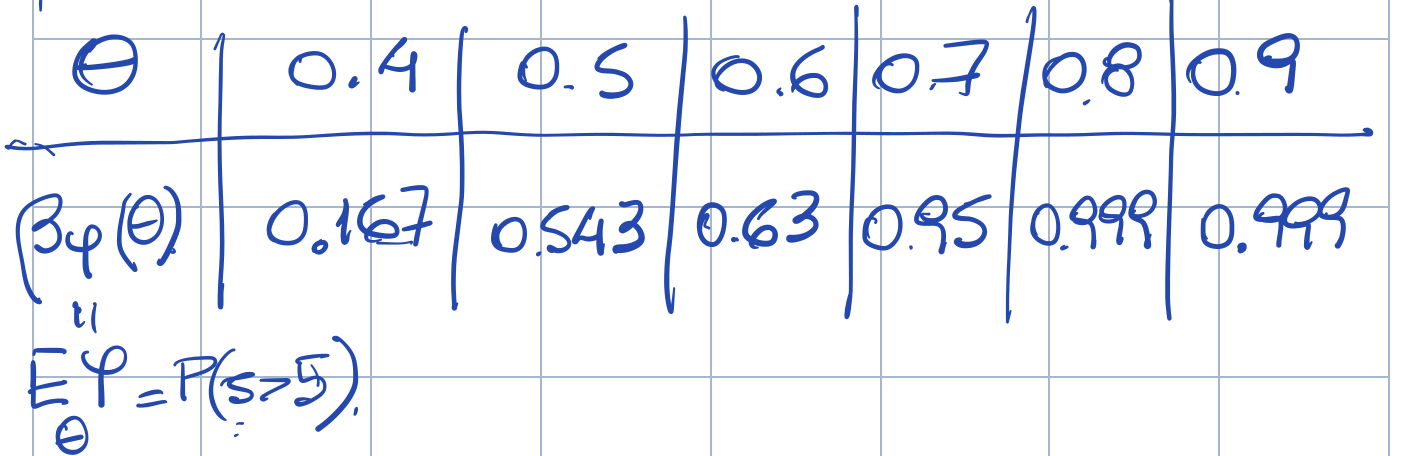
\includegraphics{Pasted image 20250726164154.png}
Que la función de potencia $\beta_\phi(\theta)$ tienda a 1 a medida que $\theta$ crece a 1 es una buena propiedad del test.
Si nos fijamos en nuestro ejemplo, el test construido se basó en el estadístico $S$, el cual recibe el nombre de \textbf{estadístico del test}.
\end{example}

\begin{remark}
Vayamos ahora al caso más sencillo posible de plantear:
\[ H_0: \mathcal{P}_0 = \{P_0\} \quad \text{vs} \quad H_1: \mathcal{P}_1 = \{P_1\} \]
(el caso de \textbf{"hipótesis simples"}).

La pregunta que queremos resolver es:
Dado $\alpha < 1$, ¿podemos encontrar un test $\phi$ de tamaño $\alpha$ tal que su potencia en $P_1$ sea mayor o igual que la potencia de cualquier otro test con nivel de significación $\alpha$?
\end{remark}

\begin{definition} Test MP
Un test $\phi$ para el problema $H_0: \mathcal{P}_0=\{P_0\}$ vs $H_1: \mathcal{P}_1=\{P_1\}$ se dice \textbf{más potente (MP)} de tamaño $\alpha$ si
\begin{itemize}
    \item i) $\beta_\phi(P_0) = \alpha$ (El tamaño del test es exactamente $\alpha$).
    \item ii) Para todo test $\phi'$ tal que $\beta_{\phi'}(P_0) \le \alpha$, se tiene que $\beta_{\phi'}(P_1) \le \beta_\phi(P_1)$.
\end{itemize}
\end{definition}

\begin{remark}
La respuesta a cómo conseguir un test MP está dada por los siguientes resultados.
\end{remark}

\begin{lemma} Neyman-Pearson I
Sea el problema de hipótesis simples planteado arriba, y sean $f_0, f_1$ las densidades de $P_0$ y $P_1$ respecto a una medida $\mu_0$.
Entonces, para cada función $0 \le \gamma(x) \le 1$ y constante $k \ge 0$, el test
$\phi: \Omega_X \to [0,1]$ definido como
\[ \phi(x) = \begin{cases} 1 & \text{si } f_1(x) > k f_0(x) \\ \gamma(x) & \text{si } f_1(x) = k f_0(x) \\ 0 & \text{si } f_1(x) < k f_0(x) \end{cases} \]
es el test más potente (MP) de tamaño $\int \phi f_0 d\mu = \beta_\phi(P_0)$.
\end{lemma}

\begin{remark}
Al cambiar $\gamma$ y $k$ siempre obtenemos un test MP, pero de tamaño $\int \phi f_0 d\mu$.
La intuición de lo que hace el test es clara en el caso discreto: el test toma el valor 1 (o sea, rechaza $H_0$) cuando la probabilidad de observar $x$ bajo la alternativa ($f_1(x)$) es $k$ veces mayor que la probabilidad de observar $x$ bajo la nula $H_0(f_0(x))$.
\end{remark}

\begin{remark}
¿Pero cómo hacemos para deducir el MP de tamaño $\alpha$ deseado?
\end{remark}

\begin{lemma} (de Neyman-Pearson II)
Para cualquier $0 < \alpha < 1$, existe un test $\phi: \Omega_X \to [0,1]$ de tamaño $\alpha$ de la forma dada en (1), con $\gamma(x) = \gamma$ (constante) y $k \in [0, \infty)$, satisfaciendo:
\[ P_0(f_1 > k f_0) \le \alpha \le P_0(f_1 \ge k f_0) \]
\[ \alpha = P_0(f_1 > k f_0) + \gamma P_0(f_1 = k f_0) \]
Más aún, si $\phi'$ es un test MP de tamaño $0 < \alpha \le 1$, entonces debe coincidir con el test $\phi$ de Neyman-Pearson salvo conjuntos de probabilidad cero, o sea:
\[ P_0(\phi \neq \phi', f_1 \neq k f_0) = 0 \]
\[ P_1(\phi \neq \phi', f_1 \neq k f_0) = 0 \]
\end{lemma}

\begin{remark}
Neyman-Pearson no especifica $\gamma(x)$, y si $\phi = \phi'$ en el conjunto $\{f_1 = k f_0\}$, realmente coinciden en todas partes salvo conjuntos de probabilidad cero.
\end{remark}

\subsection*{Tests uniformemente más potentes (UMP) para hipótesis unilaterales}

\begin{remark}
El problema al cual nos vamos a abocar es en el caso de familias paramétricas con $\Theta \subseteq \mathbb{R}$.
$\Theta = \Theta_0 \cup \Theta_1 \quad \Theta_0 = (-\infty, \theta_0] \quad \Theta_1 = (\theta_0, \infty)$
o viceversa
$\Theta_0 = [\theta_0, \infty) \quad \Theta_1 = (-\infty, \theta_0)$
Con lo cual, el problema de hipótesis sería de tipo:
$H_0: \theta \le \theta_0$ vs $H_1: \theta > \theta_0$
($H_0: \theta \ge \theta_0$ vs $H_1: \theta < \theta_0$)
(Esto es lo que llamamos \textbf{hipótesis unilaterales}).
\end{remark}

\begin{definition}
Para un problema de hipótesis $H_0: P \in \mathcal{P}_0$ vs $H_1: P \in \mathcal{P}_1$, con $\mathcal{P} = \mathcal{P}_0 \cup \mathcal{P}_1$ y $\mathcal{P}_0 \cap \mathcal{P}_1 = \emptyset$. Un test $\phi: \Omega_X \to [0,1]$ de tamaño $\alpha$ (es decir, $\sup_{P \in \mathcal{P}_0} \beta_\phi(P) = \alpha$) se dice \textbf{test uniformemente más potente de tamaño $\alpha$ (UMP-$\alpha$)} si para cualquier otro test $\phi'$ de nivel $\alpha$ ($\sup_{P \in \mathcal{P}_0} \beta_{\phi'}(P) \le \alpha$) cumple que: 
$\beta_{\phi'}(P) \le \beta_\phi(P) \quad \forall P \in \mathcal{P}_1$
\end{definition}

\begin{remark}
Volvamos a nuestro problema unilateral:
$H_0: \theta \le \theta_0$ vs $H_1: \theta > \theta_0$.

Si ponemos
$H_0: \theta = \theta_0$ vs $H_1: \theta = \theta_1$
con $\theta_1 > \theta_0$, sabemos encontrar el test MP.
\end{remark}

\begin{example}
Sea $X \sim \text{Bi}(n, \theta)$, con $0 < \theta < 1$.
El problema de hipótesis es
$H_0: \theta = \theta_0$ vs $H_1: \theta = \theta_1$, con $\theta_1 > \theta_0$.
Si aplicamos el test de Neyman-Pearson:
$\phi(x) = \begin{cases} 1 & \text{si } f_1(x) > k f_0(x) \\ \gamma & \text{si } f_1(x) = k f_0(x) \\ 0 & \text{si } f_1(x) < k f_0(x) \end{cases}$
donde el cociente de verosimilitudes es:
$L(x) = \frac{f_1(x)}{f_0(x)} = \frac{\binom{n}{x} \theta_1^x (1-\theta_1)^{n-x}}{\binom{n}{x} \theta_0^x (1-\theta_0)^{n-x}} = \left(\frac{\theta_1}{\theta_0}\right)^x \left(\frac{1-\theta_1}{1-\theta_0}\right)^{n-x}$
Como $\theta_1 > \theta_0$, tenemos que $a = \frac{\theta_1}{\theta_0} > 1$ y $b = \frac{1-\theta_1}{1-\theta_0} < 1$.

O sea, el test se puede escribir como:
$\phi(x) = \begin{cases} 1 & \text{si } L(x) > k \\ \gamma & \text{si } L(x) = k \\ 0 & \text{si } L(x) < k \end{cases}$
$k$ se determina por la condición de nivel:
$P_0(L(x) > k) \le \alpha \le P_0(L(x) \ge k)$
y $\gamma$ por la ecuación
$\alpha = P_0(L > k) + \gamma P_0(L=k)$.
Trabajemos la región $L > k$:
$L > k \leftrightarrow \log L > \log k$
$x \log a + (n-x) \log b > \log k$
$x(\log a - \log b) > \log k - n \log b$
Como $\log a > 0$ y $\log b < 0$, entonces $\log a - \log b > 0$, y la desigualdad se mantiene:
$x > \frac{\log k - n \log b}{\log a - \log b} =: m$

$P(L > k) = P(X > m)$. Luego el test $\phi$ toma la forma:
$\phi(x) = \begin{cases} 1 & \text{si } x > m \\ \gamma & \text{si } x = m \\ 0 & \text{si } x < m \end{cases}$
donde $m$ y $\gamma$ satisfacen:
$P_0(X > m) \le \alpha \le P_0(X \ge m)$
$\alpha = P_0(X > m) + \gamma P_0(X=m)$
Luego, el test obtenido sólo depende de $\theta_0$ y no depende de $\theta_1$, con lo cual resulta el test más potente (MP) para cualquiera sea la alternativa $\theta_1 > \theta_0$. Luego, es el \textbf{test uniformemente más potente de tamaño $\alpha$ (UMP-$\alpha$)} para el problema de hipótesis:
$H_0: \theta = \theta_0$ vs $H_1: \theta > \theta_0$.
\end{example}

\begin{example}
Sea $X_1, \dots, X_n$ una muestra aleatoria i.i.d. tal que $X_1 \sim N(\theta, 1)$.
Sea el problema de hipótesis $H_0: \theta = \theta_0$ vs $H_1: \theta > \theta_0$.
Ver que el test UMP-$\alpha$ es de la forma:
$\phi(X_1, \dots, X_n) = \begin{cases} 1 & \text{si } \frac{\sum X_i}{n} > m \\ 0 & \text{si } \frac{\sum X_i}{n} \le m \end{cases}$
donde $m$ cumple:
$P_0(\bar{X}_n > m) \le \alpha \le P_0(\bar{X}_n \ge m)$
$\alpha = P_0(\bar{X}_n > m)$.

Esto que se ve en los ejemplos, puede ser generalizado a través de la propiedad siguiente:
\end{example}

\begin{definition}
Sea la familia de distribuciones $\mathcal{P} = \{P_\theta : \theta \in \Theta \subseteq \mathbb{R}\}$ dominadas por una medida $\mu$, y sean $f_\theta$ sus densidades.
La familia de densidades $\{f_\theta : \theta \in \Theta\}$ se dice que tiene \textbf{cociente de verosimilitud monótono (CVM)} en un estadístico $T: \Omega_X \to \mathbb{R}$ si para todo $\theta_1 < \theta_2$, con $\theta_1, \theta_2 \in \Theta$. El cociente de verosimilitud:
$L(x) = \begin{cases} \frac{f_{\theta_2}(x)}{f_{\theta_1}(x)} & \text{si } f_{\theta_1}(x) > 0 \\ \infty & \text{si } f_{\theta_1}(x) = 0 \text{ y } f_{\theta_2}(x) > 0 \end{cases}$
es una función monótona (creciente o decreciente) en $T(x)$.
(El cociente de verosimilitud no se define si $f_{\theta_1}(x) = 0 = f_{\theta_2}(x)$).
\end{definition}

\begin{example}
Sea $X_1, \dots, X_n$ una muestra aleatoria i.i.d. con $X_1 \sim U(0, \theta)$.
En este caso, el espacio paramétrico es $\Theta = (0, \infty)$.
La densidad conjunta es:
$f_\theta(x_1, \dots, x_n) = \frac{1}{\theta^n} I_{(0, \infty)}(\min x_i) I_{[0, \theta]}(\max x_i)$
¿Es esta familia de CVM?
Sean $0 < \theta_1 < \theta_2$. El cociente de verosimilitud es:
$\frac{\frac{1}{\theta_2^n} I_{[0, \theta_2]}(\max x_i)}{\frac{1}{\theta_1^n} I_{[0, \theta_1]}(\max x_i)} = \begin{cases} 0 & \text{si } \max x_i > \theta_2 \\ (\frac{\theta_1}{\theta_2})^n & \text{si } \max x_i \le \theta_1 \\ \infty & \text{si } \theta_1 < \max x_i < \theta_2 \end{cases}$

Luego, tiene CVM en el estadístico $T(X_1, \dots, X_n) = X_{(n)}$.
\end{example}

\begin{remark}
A continuación vamos a enunciar un lema, que va a permitirnos después obtener el test UMP-$\alpha$ en el problema de hipótesis unilaterales.
\end{remark}

\begin{lemma}
Sea $\Theta \subseteq \mathbb{R}$ y supongamos que tenemos la familia de densidades $\{f_\theta : \theta \in \Theta\}$ respecto de la medida $\mu$, que cumple la propiedad de CVM en el estadístico $T(x)$. Sea además el test $\phi$ de Neyman-Pearson II, que depende del cociente de verosimilitud. Si esta es una función creciente (decreciente) en $T$, entonces se cumple que la función potencia
$\beta_\phi(\theta) = E_\theta(\phi) = \int \phi f_\theta d\mu$
es creciente (decreciente).
\end{lemma}

\begin{remark}
Ahora llegamos al enunciado del teorema que nos dará los test UMP-$\alpha$ en el problema unilateral.
\end{remark}

\begin{theorem}
Sea la familia de densidades $\{f_\theta : \theta \in \Theta \subseteq \mathbb{R}\}$ con CVM creciente en el estadístico $T$. Sea $0 < \alpha < 1$, $\theta_0 \in \Theta$, y $P_0(B) = \int_B f_{\theta_0} d\mu$.
\begin{itemize}
    \item a) Sea el problema de hipótesis
    $H_0: \theta \le \theta_0$ vs $H_1: \theta > \theta_0$.
    Entonces el test definido como
    $\phi(x) = \begin{cases} 1 & \text{si } T(x) > k \\ \gamma & \text{si } T(x) = k \\ 0 & \text{si } T(x) < k \end{cases}$
    donde $k, \gamma \in$ satisfacen que
    $P_0(T>k) \le \alpha \le P_0(T \ge k)$
    $\alpha = P_0(T>k) + \gamma P_0(T=k)$
    es un test UMP-$\alpha$ para el problema de hipótesis.
    \item b) Sea el problema de hipótesis
    $H_0: \theta \ge \theta_0$ vs $H_1: \theta < \theta_0$.
    Entonces el test definido como
    $\phi'(x) = \begin{cases} 1 & \text{si } T(x) < k' \\ \gamma' & \text{si } T(x) = k' \\ 0 & \text{si } T(x) > k' \end{cases}$
    donde $k', \gamma' \in$ satisfacen que
    $P_0(T < k') \le \alpha \le P_0(T \le k')$
    $\alpha = P_0(T < k') + \gamma' P_0(T=k')$
    es un test UMP-$\alpha$ para el problema de hipótesis.
\end{itemize}
\end{theorem}

\begin{remark}
¿Es posible encontrar un test UMP-$\alpha$ para problemas de hipótesis del tipo $H_0: \theta = \theta_0 \text{ vs } H_1: \theta \neq \theta_0$?
(Problema de \textbf{hipótesis bilateral}).
\end{remark}

\begin{example}
Sea $X \sim \text{Bi}(n, \theta)$, con $0 < \theta < 1$.
Y tenemos el problema de hipótesis:
$H_0: \theta = 0.5 \text{ vs } H_1: \theta \neq 0.5$.
¿Podemos encontrar un test UMP-$\alpha$ para este problema?
Si uno plantea el problema unilateral:
$H_0: \theta=0.5 \text{ vs } H_1^+: \theta > 0.5$.
Para este problema sabemos encontrar el test UMP-$\alpha$, que es de la forma:
$\phi^+(x) = \begin{cases} 1 & \text{si } x > k^+ \\ \gamma^+ & \text{si } x = k^+ \\ 0 & \text{si } x < k^+ \end{cases}$
donde $k^+$ y $\gamma^+$ se determinan para asegurar que $\alpha = E_{0.5}[\phi^+(X)]$.

Si uno considera el problema:
$H_0: \theta=0.5 \text{ vs } H_1^-: \theta < 0.5$.
% 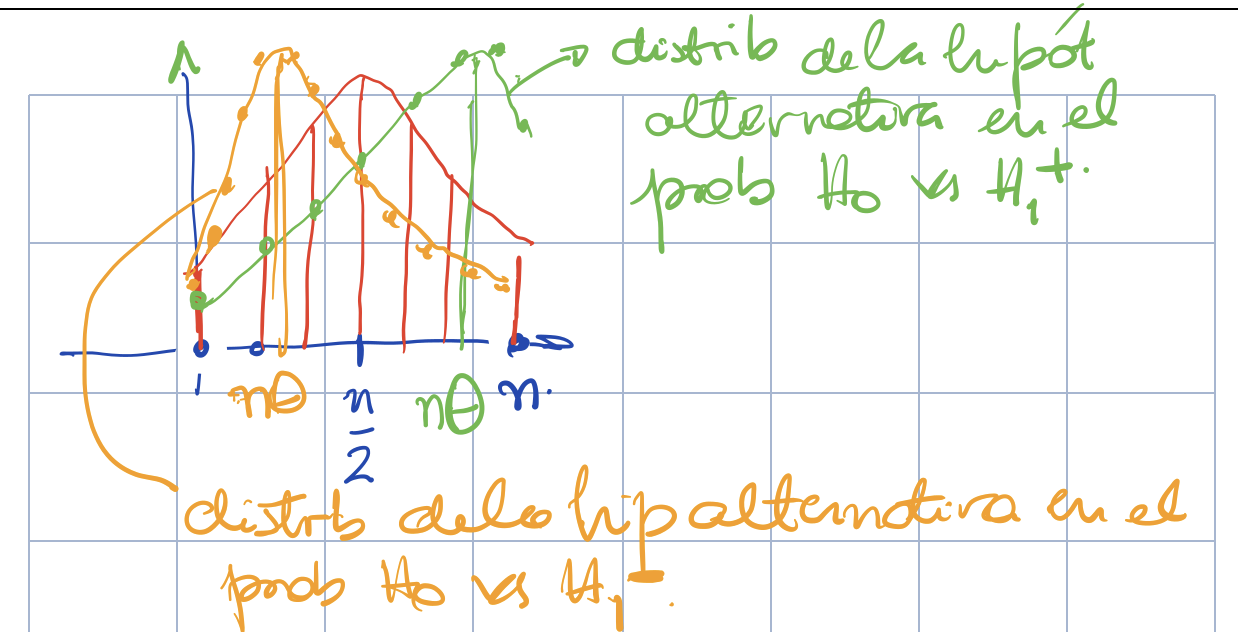
\includegraphics{Pasted image 20250726170614.png}
El test MP para $H_0$ vs $H_1^-$ es de la forma:
$\phi^-(x) = \begin{cases} 1 & \text{si } x < k^- \\ \gamma^- & \text{si } x = k^- \\ 0 & \text{si } x > k^- \end{cases}$
donde $\gamma^-$ y $k^-$ se eligen de forma tal que $\alpha = E_{0.5}[\phi^-(X)]$.

Supongamos que tenemos el test UMP-$\alpha$ para el problema bilateral, y lo llamamos $\phi^0$.
Entonces, $\phi^0$ es el más potente para el problema de hipótesis $H_0: \theta=0.5 \text{ vs } H_1^+: \theta > 0.5$.
Esto implica que las funciones de potencia deben ser iguales:
$\beta_{\phi^0}(\theta) = \beta_{\phi^+}(\theta) \quad \forall \theta \ge 0.5$
$\implies E_\theta[\phi^0(X)] = E_\theta[\phi^+(X)] \quad \forall \theta \ge 0.5$

Sea $g^+(x) = \phi^0(x) - \phi^+(x)$. Entonces:
$0 = E_\theta[g^+(X)] = \sum_{j=0}^n g^+(j) \binom{n}{j} \theta^j (1-\theta)^{n-j} \quad \forall \theta \ge 0.5$
$0 = (1-\theta)^n \sum_{j=0}^n g^+(j) \binom{n}{j} \left(\frac{\theta}{1-\theta}\right)^j$

Si $\theta \in [0.5, 1)$, entonces $\eta = \frac{\theta}{1-\theta} \in [1, \infty)$.
Luego, tenemos un polinomio de grado $n$ en $\eta$ que sobre la semirrecta $[1, \infty)$ se anula. 
...es el polinomio nulo, lo que implica que sus coeficientes son cero:
$g^+(j) = 0 \quad \forall j \in \{0, \dots, n\}$
$\implies \phi^0(j) = \phi^+(j) \quad \forall j \in \{0, \dots, n\}$

Ahora, si consideramos el problema $H_0: \theta=0.5 \text{ vs } H_1^-: \theta < 0.5$ y definimos $g^-(j) = \phi^0(j) - \phi^-(j)$, de la misma forma concluimos que
$\phi^0(j) = \phi^-(j) \quad \forall j \in \{0, \dots, n\}$

Juntando ambos resultados, tendríamos $\phi^-(j) = \phi^+(j)$ para todo $j$.
Lo cual es imposible, porque sabemos la forma de los tests $\phi^+$ y $\phi^-$.

$\implies$ \textbf{NO existe el test UMP-$\alpha$ para el problema bilateral.}

Como no podemos plantear procedimientos óptimos, ¿qué podemos hacer?
\end{example}

\end{document}
